
\chapter{ Compodoc }
Compodoc is an automated documentation tool for your Angular application. For small apps, having documentation can feel like overkill. However, when your app grows and the size of your team increases, good documentation practices from the get-go can save developers from wasted time and overlapping code. 

Having a documentation tool within your app is incredibly important. Why? It increases visibility in the following areas:

\begin{enumerate}
  \item Overview 
  \item Dependencies
  \item Various types of Modules, Components, Services etc. 
  \item Routes
  \item Documentation coverage
\end{enumerate}

Why compodoc? Because it is the most comprehensive and easiest to work with when it comes to auto generating documentation. It is also open sourced and generates a static documentation of your application. 

Here's how you install and use compodoc.

\section{ Installing Compodoc }
\begin{verbatim}
npm install -g @compodoc/compodoc --save-dev
\end{verbatim}

\section{ Adding to package.json }
To ensure that compodoc gets shipped between team members and works as expected, add compodoc to your package.json file. 

\begin{verbatim}
  "compodoc": "compodoc -p tsconfig.json",
  "compodoc-serve": "compodoc -s tsconfig.json",
\end{verbatim}

Now if we want to generate documentation, and we are in development mode, we can simply run:
\begin{verbatim}
npm run compodoc-serve  
\end{verbatim}

\section{Overview - Using Compodoc to Remove Dead Code}
Compodoc has a section called overview. It allows you to see all of your modules, components, and services. By doing so, you can see how they all feed into each other. 

\begin{figure}
\caption{Compodoc overview}
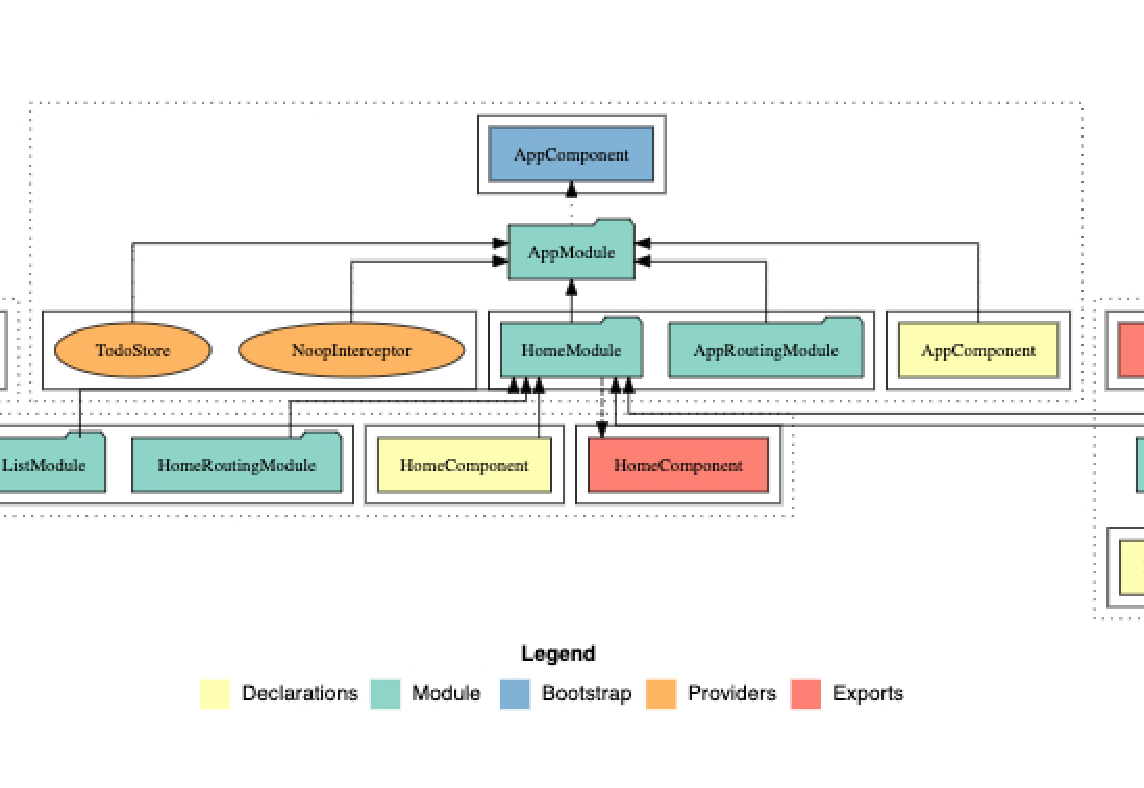
\includegraphics[width=414pt]{graphics/compodoc/compodoc-overview-screenshot.pdf}
\end{figure}

In the above image, we can see how Compodoc works. The tree structure allows us to see which components are feeding into which modules. If there are too many lines, then it means that your app may need to be refactored for a cleaner workflow. Stand alone components with no attached modules is often a sign of dead code, which means it can be cleaned through deletion. 


\section{Dependencies}
Seeing what dependencies your app is using is as simple as going to your \lstinline{package.json} file. However, if you've got more than a barebones Angular app, the file is not visually appealing to look at. It's hard to see how everything is interconnected with one another. 

Compodoc solves this issue by creating a visual output. This allows us to quickly capture relationships without having to slow down and manually figure things out. 

\begin{figure}
\caption{Compodoc overview}
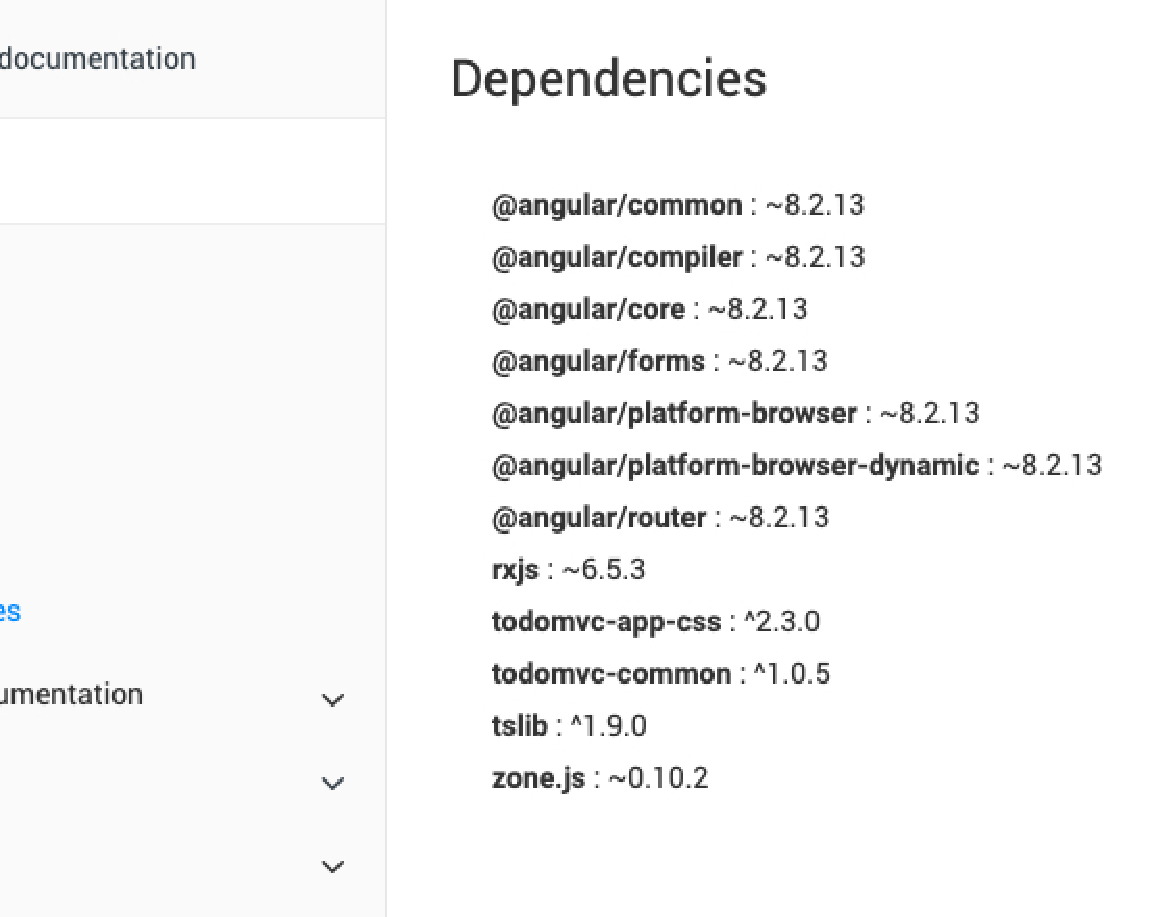
\includegraphics[width=414pt]{graphics/compodoc/dependencies/compo-dependencies-screenshot.pdf}
\end{figure}


\lstinline{package.json} has a way of creeping up on a project, making it hard to navigate. With compodoc, your meta information is presented in a way that's easier to mentally digest. 

\section{Various Types of Modules, Components etc.}
Compodoc provide dropdowns of all modules, components, classes, services, interceptors, guards, interfaces, and miscellaneous within app.

This is good for two reasons: 
\begin{enumerate}
  \item It lays everything out. There is no secrets, or hidden surprises. You know exactly what's going on within the app. 
  \item Defines everything within your app - including but not limited to interceptors, guards, and interfaces. This information is good in team settings, where members may be working on islands of code that may need to connect to and impact on pieces created by others. 
\end{enumerate}

\begin{figure}
\caption{Compodoc navigation of Modules, Components, etc.}
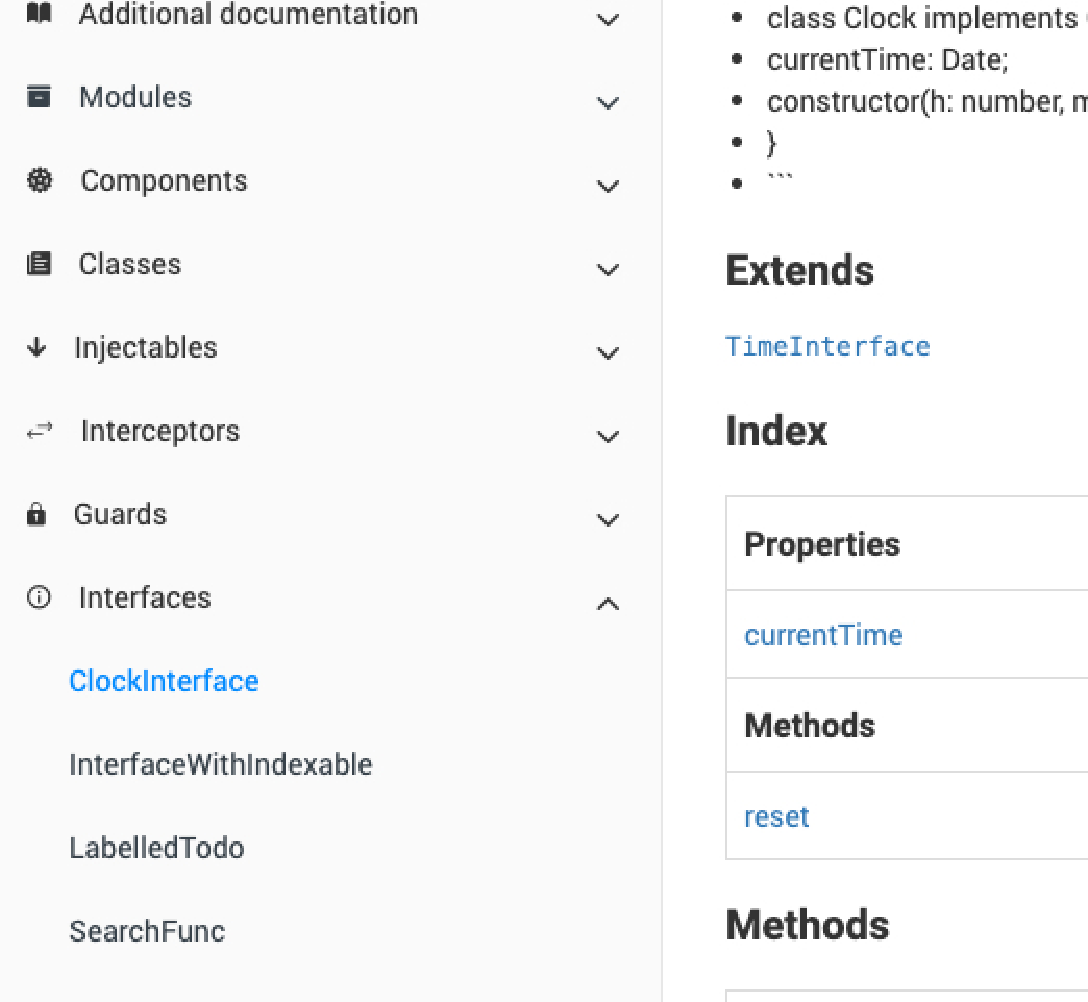
\includegraphics[width=414pt]{graphics/compodoc/nav/compodoc-nav-screenshot.pdf}
\end{figure}

\section{Routes}
Compodoc also gives you the ability to visualize the routes that are in your application, and which components are attached. This is useful for large applications. The visualization also lets you mock the relationships and help you see how the parts of your app is connected to one another. 

\begin{figure}
\caption{Compodoc Routes Example}
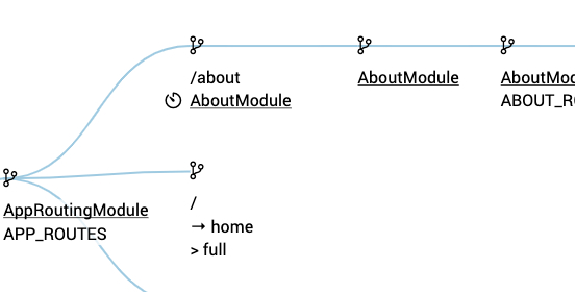
\includegraphics[width=414pt]{graphics/compodoc/routes/compodoc-routes.pdf}
\end{figure}

You can also click through the routes. With compodoc, your documentation becomes a meta living document that can help speed up your workflow by turning your meta information into something visual.


\section{Documentation Coverage}
Compodoc compiles documentation in one place. In contrast to other available frameworks, this is a major perk because it gives you the bigger picture approach to your application, while still having the ability to drill down into the finer points. 

For example, if you have a method within a component that looks something like this: 

\begin{lstlisting}
/**
  * Display only completed todos
  */
displayCompleted() {
  this.currentFilter = 'completed';
  EmitterService.get(this.id).emit('displayCompleted');
}
/**
  * Display all todos
  */
displayAll() {
  this.currentFilter = 'all';
  EmitterService.get(this.id).emit('displayAll');
}
\end{lstlisting}

\begin{figure}
\caption{Compodoc Documentation Example}
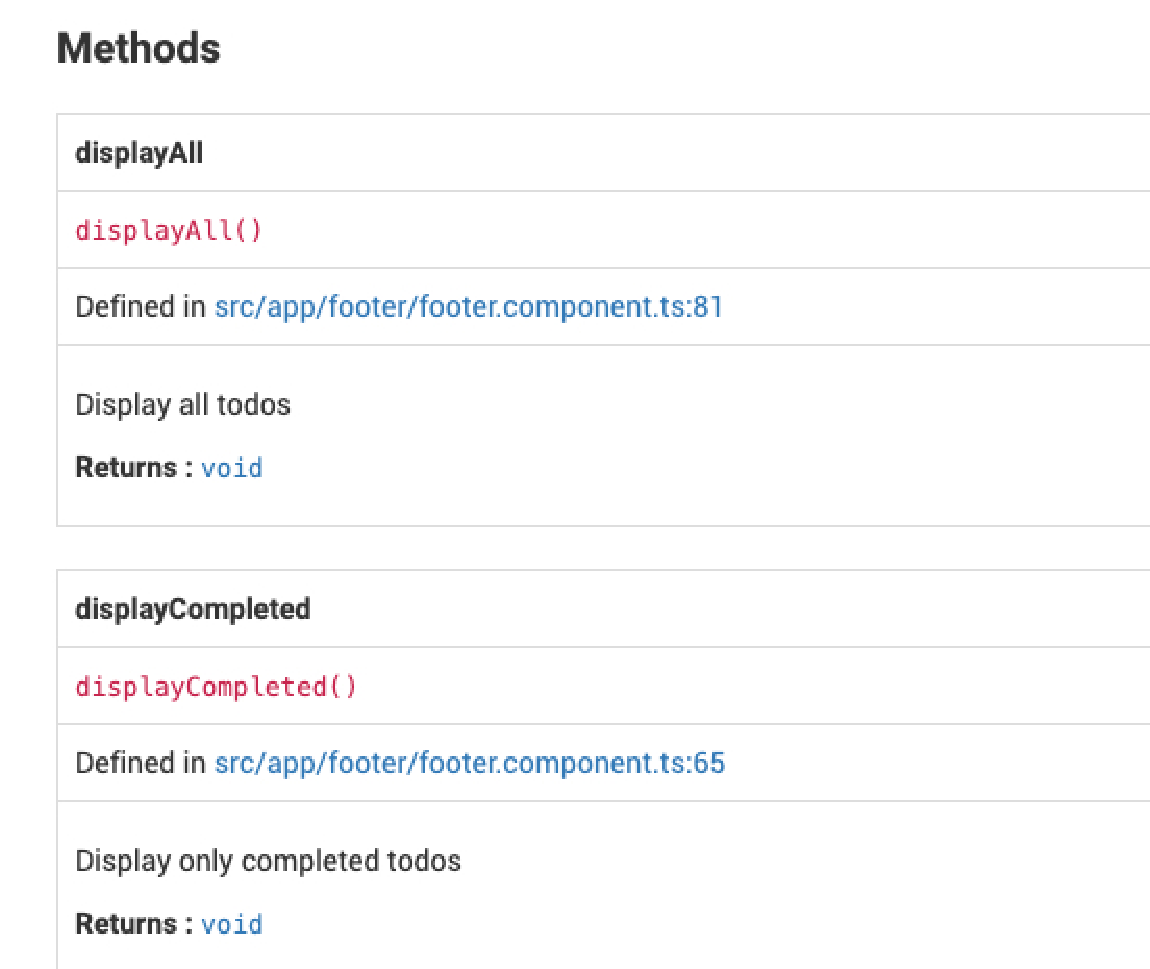
\includegraphics[width=414pt]{graphics/compodoc/documentation/documentation-coverage.pdf}
\end{figure}

Compodoc will take the JsDoc documentation and generate it in a way that is simple to navigate. 

\section{Pushing Documentation to Staging Area }
As we did initially, is that we created a two npm scripts. One of them for compodoc development, and the other compodoc production.

By running the following, you can generate documentation in your default output folder.
 
\begin{lstlisting}
"compodoc": "compodoc -p tsconfig.json",
\end{lstlisting}

This link can be pushed and bundled with your project so that everyone has access to it. 
